%%%%%%%%%%%%%%%%%%%%%%%%%%%%%%%%%%%%%%%%%%%%%%%%%%%%%%%%%%%%%%%%%%%%%%%%%%%%%%%%
%2345678901234567890123456789012345678901234567890123456789012345678901234567890
%        1         2         3         4         5         6         7         8

\documentclass[letterpaper, 11 pt]{article}  % Comment this line out
                                                          % if you need a4paper
%\documentclass[a4paper, 10pt, conference]{ieeeconf}      % Use this line for a4
                                                          % paper
\usepackage{url}
\usepackage{graphicx}
\usepackage{amsmath}
\usepackage{amssymb}
\usepackage{amsfonts}
\usepackage{proof}
\usepackage{tikz}
\usepackage[margin=1.2in]{geometry}


\usepackage{color}
\definecolor{light-gray}{gray}{0.95}
\usepackage{listings}
\lstset{ %
language=Python,                % choose the language of the code
basicstyle=\footnotesize,       % the size of the fonts that are used for the code
numbers=left,                   % where to put the line-numbers
numberstyle=\footnotesize,      % the size of the fonts that are used for the line-numbers
stepnumber=1,                   % the step between two line-numbers. If it is 1 each line will be numbered
numbersep=5pt,                  % how far the line-numbers are from the code
backgroundcolor=\color{light-gray},  % choose the background color. You must add \usepackage{color}
showspaces=false,               % show spaces adding particular underscores
showstringspaces=false,         % underline spaces within strings
showtabs=false,                 % show tabs within strings adding particular underscores
frame=single,           % adds a frame around the code
tabsize=2,          % sets default tabsize to 2 spaces
captionpos=b,           % sets the caption-position to bottom
breaklines=true,        % sets automatic line breaking
breakatwhitespace=false,    % sets if automatic breaks should only happen at whitespace
escapeinside={\%*}{*)}          % if you want to add a comment within your code
}



\title{Common Instruction-Level Abstraction Issues}
\author{}

\date{Draft Working Document: \today}

\begin{document}
\maketitle

\providecommand{\bd}[0]{\mathbb{B}}
\providecommand{\st}[1]{\mathrm{#1}}
\providecommand{\ft}[1]{\mathtt{#1}}

%In this document, we will show readers how ILA can be used to model different designs. Because we will show some example templates, we assume the readers are already familiar with the ILA definition and the syntax of writing a template. 

%%%%%%%%%%%%%%%%%%%%%%%%%%%%%%%%%%%%%%%%%%%%%%%%%%%%%%%%%%%%%%%%%%%%%%%%%%%%%%%%
%2345678901234567890123456789012345678901234567890123456789012345678901234567890
%        1         2         3         4         5         6         7         8

\documentclass[letterpaper, 11 pt]{article}  % Comment this line out
                                                          % if you need a4paper
%\documentclass[a4paper, 10pt, conference]{ieeeconf}      % Use this line for a4
                                                          % paper
\usepackage{url}
\usepackage{graphicx}
\usepackage{amsmath}
\usepackage{amssymb}
\usepackage{amsfonts}
\usepackage{proof}
\usepackage{tikz}
\usepackage[margin=1.2in]{geometry}


\usepackage{color}
\definecolor{light-gray}{gray}{0.95}
\usepackage{listings}
\lstset{ %
language=Python,                % choose the language of the code
basicstyle=\footnotesize,       % the size of the fonts that are used for the code
numbers=left,                   % where to put the line-numbers
numberstyle=\footnotesize,      % the size of the fonts that are used for the line-numbers
stepnumber=1,                   % the step between two line-numbers. If it is 1 each line will be numbered
numbersep=5pt,                  % how far the line-numbers are from the code
backgroundcolor=\color{light-gray},  % choose the background color. You must add \usepackage{color}
showspaces=false,               % show spaces adding particular underscores
showstringspaces=false,         % underline spaces within strings
showtabs=false,                 % show tabs within strings adding particular underscores
frame=single,           % adds a frame around the code
tabsize=2,          % sets default tabsize to 2 spaces
captionpos=b,           % sets the caption-position to bottom
breaklines=true,        % sets automatic line breaking
breakatwhitespace=false,    % sets if automatic breaks should only happen at whitespace
escapeinside={\%*}{*)}          % if you want to add a comment within your code
}


\title{ILA Modeling of Timing}
\author{}

\date{Draft Working Document: \today}

\begin{document}
\maketitle

\providecommand{\bd}[0]{\mathbb{B}}
\providecommand{\st}[1]{\mathrm{#1}}
\providecommand{\ft}[1]{\mathtt{#1}}

%%%%%%%%%%%%%%%%%%%%%%%%%%%%%%%%%%%%% Body %%%%%%%%%%%%%%%%%%%%%%%%%%%%%%%%%%%%%
% Section on how to use ILA to handle clock and timing issues.

\section*{Timing}


Instruction-Level Abstraction can be used to abstract away timing information if they are not intended by the specification. However if timing requirements are part of specification, ILA can also be used to capture the timing on the interface at a scale of clock cycles.

\begin{figure}[h]
\caption{Timing diagram of burst write in an example bus}
\label{fig:timing}
\centering
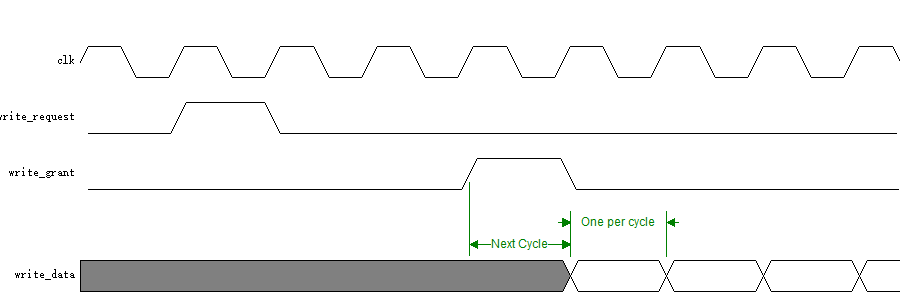
\includegraphics[width=\textwidth]{images/timing.png}
\end{figure}

Let's take a simple bus interface as an example. An accelerator can initiate a burst write of an arbitrary length, it first sends a request to the bus arbiter and waits for the grant. The grant can come any time after the request. But right after the grant the accelerator should sends the data on the data port one per cycle. So there is timing requirement between grant and data write. The timing diagram is shown in Figure \ref{fig:timing}. An example template of the write interface is shown below. The key idea in modeling timing charateristic is to use a counter to count the cycle. And when writing the refinement relations, define the matching between the behavior of the implementation in each cycle with each step in the sub-instructions in ILA.


\lstinputlisting{code/timingExample.py}

%\bibliography{refs}
%\bibliographystyle{unsrt}

\end{document}



% Section on how to use ILA to specify instruction ordering.

\section*{Instruction Ordering}


% Section on how to use ILA to model interrupts.

\section*{Interrupt}



% Section on what is the difference between micro and sub instructions.
% Detail about the relation between micro-architecture and specification.

\section*{Specification and Micro-architecture}


\section*{Concurrency}

In this scenario we consider two different design options: physical and logical multi-core (logical is simultaneous multithreading). 
\subsection*{Physical multi-core} 
In a physical multi-core design computational resources are duplicated. Modern CPUs contain 2-24 physical cores, while GPUs contain thousands of physical cores. Since our hierarchical-ILA supports concurrent execution of instructions, it can be used to model such multi-core designs. More precisely, an ILA for a multi-core design includes many identical child-ILAs. Note that while multi-core designs are based on the notion of duplicating computational resources, the way they operate is different. The most obvious example is CPU vs. GPU. In most cases, execution on different GPU cores is independent, unlike the case of a CPU. We need to decide if we add this modeling power to the ILA.

\subsection*{Logical multi-core, aka SMT, HyperThreading}
In this case, the computational resources are not duplicated. Instead, the architectural state (e.g. control and general purpose registers) are duplicated. Using this approach, if the CPU includes one core, the OS views it as two \emph{logical} cores. The management of the physical core (the actual computational resource) is done at the hardware level, i.e., by the CPU and can be captured by the ILA.

%\bibliography{refs}
%\bibliographystyle{unsrt}

\end{document}

